% File name: documentation.tex
% Date:      13.12.2011 16:13
% Authors:   Radek Fér          <xferra00@stud.fit.vutbr.cz>
%            Miroslav Paulík    <xpauli00@stud.fit.vutbr.cz>

\documentclass[a4paper,12pt,titlepage]{article}
\usepackage[czech]{babel}
\usepackage{color}
\usepackage{tabularx}
\usepackage{hyperref}
\usepackage[utf8]{inputenc}
\usepackage[left=2cm, top=3cm, text={17cm, 24cm}]{geometry}
\usepackage{graphicx} % for .eps images
\usepackage{fancyvrb,fancybox,calc}
\usepackage[svgnames]{xcolor}
 
\hypersetup{linktoc=all}
%\hypersetup{pdfborder={0 0 0 [0 0]}
\hypersetup{colorlinks=true}
\hypersetup{linkcolor=blue}

% European layout (no extra space after `.')
\frenchspacing

% no indent, free space between paragraphs
\setlength{\parindent}{0pt}
\setlength{\parskip}{1ex plus 0.5ex minus 0.2ex}

\begin{document}
\renewcommand{\refname}{Literatura}

\title{\LARGE Pokus o vytvoření jednoduchého 3D \uv{myšítka} \\
       {\large Projektová dokumentace do předmětu ITU 2011/12}}
\author{ \begin{tabularx}{\textwidth}{X r l X}
& Radek Fér & \texttt{xferra00@stud.fit.vutbr.cz} & \\
& Miroslav Paulík & \texttt{xpauli00@stud.fit.vutbr.cz} & \\
\end{tabularx}
}
\date{\today, FIT VUT Brno}

\maketitle

\newpage

\thispagestyle{empty}
\tableofcontents
\newpage
\setcounter{page}{1}

% \label{summary}
% \cite{citId}
% \url{www.google.com}

%\begin{figure}[htb]
%\centering
%\includegraphics[width=0.8\textwidth]{img/myplot.eps}
%\caption{Mycaption}
%\label{fig:myplot}
%\end{figure}

\section{Úvod}\label{intro}
Tento projekt si klade za cíl odzkoušet možnosti využití speciálního
vstupního zařízení (zkonstruovaného podle myšlenky jednoho z autorů),
které {\bf využívá 2 dostupná 2D polohovací zařízení (myš, touchpad, \ldots)
k vytvoření jednoho 3D polohovacího zařízení}. A to tak, že pohyby
oněch dvou 2D polohovacích zařízení jsou slučovány do pohybů nad 3D.

Dále si projekt klade za cíl navrhnout a otestovat různá uživatelská rozhraní
využívající tohoto zařízení tak, aby se práce s virtuálním 3D prostorem
stala více efektivnější, intuitivnější a příjemnější.

% File name: navrh.tex
% Date:      13.12.2011 17:00

\section{Návrh}

% File name: implementace.tex
% Date:      13.12.2011 17:00

\section{Implementace}

\subsection{Overview}

\subsection{Merging}\label{merging}


\subsection{Knihovny}
GLUT, SDL

\subsection{Omezení naší implementace}

- Pouze Linux



% File name: experimenty.tex
% Date:      13.12.2011 17:00

\section{Experimenty a testování}
Cílem experimentální části je získání užitečných informací o testovaném subjektu a z nich vycházející další vývoj. Tato kapitola bude tedy popisovat stategii testování a experimentů na rozhraní m2m, výběr vhodné skupiny účastníků těchto pokusů a popisem jednotlivých experimentů a analýzy jejich výsledků.

\subsection{Strategie experimentování a testování}
Úplně jako první bylo potřeba zjistit, jakým způsobem by měla být aplikace ovládána, které tlačítka obou polohovacích zařízení se budou používat ke kterým činnostem a jak správně nastavit osy pohybu každého ze vstupních zařízení. Jelikož má rozhraní pracovat v prostředí 3D, musí navíc existovat prostředek pro prostorovou orientaci. Cílem prvního experimentu se tedy stalo zjištění reakcí uživatelů na různé možnosti ovládání prostorového kurzoru a jeho přizpůsobení při operaci otáčení 3D scény. Získání výše zmíněných informací umožnilo vytvořit několik demonstračních aplikací, jež se později staly instruktážními nástroji pro poslední experiment. Než k němu ale došlo, byl proveden pilotní test celé sady instruktážních aplikací kvůli zjištění možných nedostatků ještě před samotným testováním. Cílem celého procesu experimentování a testování však bylo hlavně získání údajů o míře efektivnosti práce s rozhraním m2m. A právě to bylo náplní závěrečného experimentu. 

\subsubsection{Výběr účastníků experimentů}
Největší vliv na výběr skupiny testujících uživatelů byla jejich schopnost pracovat s počítačem, uživatel mající problém obsluhovat jedno polohovací zařízení bude jistě mít problém i se zařízením druhým. Proto jsme požádali o účast v experimentování skupinu 25-ti vysokoškolských studentů, kteří s požadavkem běžného ovládání počítače nemají problém.

\subsubsection{Experiment č. 1 - Požadavky na ovládání a orientaci v 3D prostředí}
Jak již bylo uvedeno výše, cílem prvního experimentu bylo nalezení optimálního ovládání a zjištění dalších možných nastavení, které by si eventuálně uživatel mohl explicitně zvolit. Jako forma získání informací byl zvolen dotazník. Ten byl rozdělen na 2 části. První byla zaměřena na informace o dotazované osobě a jejich zkušenostech s prací v 3D, zatímco druhá na jejich očekávání ohledně práce s 3D objekty.

\noindent Přehled důležitých dotazů a vyhodnocení jejich odpovědí:

\noindent Preferujete stejnou funkcionalitu tlačítek na obou polohovacích zařízeních?\\
Odpovědi: ANO (25x), NE (0x).

\noindent Které tlačítko preferujete pro natáčení scény?\\
Odpovědi: LEVÉ (0x), PROSTŘEDNÍ (21x), PRAVÉ (4x).

\noindent Preferujete obrácený pohyb myši (posun myši vlevo znamená posun vpravo na obrazovce) před pohybem shodným?\\
Možné odpovědi: ANO (7x), NE (18x).

\noindent Preferujete obrácený význam levého a pravého tlačítka u druhého polohovacího zařízení?\\
Možné odpovědi: ANO (4x), NE (21x).

Z odpovědí, které byly většinově přikloněny k jedné z možností, vyplynuly požadavky pro ovládání polohovacích zařízení. Velmi překvapivě dopadl dotaz na obrácení významu levého a pravého tlačítko vzhledem opačnému pořadí prstů na druhé lidské ruce. Bylo možné očekávat, že se dozazující budou upřednostňovat stejný význam tlačítka ovládaného ukazováčkem stejně jako u druhé ruky. Výsledky průzkumu však ukázaly, že tomu tak být nemusí. 

\subsubsection{Pilotní testování}
V rámci ověření správné funkčnosti instruktážních aplikací bylo provedeno pilotní testování. Tohoto se zúčastnili pouze 2 dobrovolníci, kteří však nepatřili do skupity účastníků prvního a závěrečného experimentu. Tito dobrovolníci však velmi důsledně připomínkovaly každou nejasnost a hlásily každou nalezenou chybu. Na základě jejich poznámek k funkcionalitě byl implementován např. tzv \uv{spinning mód} umožňující automatickou rotaci kamery, která umožní snažší orientaci v 3D prostoru aniž by bylo nutné explicitně natáčet scénu. Dále bylo upraveno zvýraznění zaměření objektu v měřeném testu nebo vyladěn způsob, jakým uživatel měnil nastavení polohovacích zařízení.

\subsubsection{Experiment č. 2 - Efektivnost práce s rozhraním m2m}
Cílem závěrečného pokusu bylo demonstrovat rychlost práce s rozhraním m2m a to měřením času potřebného ke splnění úkolu. Před samotným měřením byli všichni účastníci experimentu seznámeni s ovládáním ve třech demonstračních aplikacích, které sloužili k vyzkoušení práce v 3D prostředí a nastavení ovládání. Po tomto seznámení s prostředím byl každému zúčastněnému spuštěn test v podobě aplikace 3D moorhuhn, kde byl měřen čas \uv{zastřelení} 50-ti krychlí umístěných v 3D prostoru.

V tomto experimentu byly měřeny časy mezi jednotlivými zásahy a ty pak byly dále zpracovány. Všechny hodnoty byly interpolovány do přímky, jež znázorňovala relativní zrychlení při změřování a zásahu cíle. Následující obrázek ukazuje, že rychlost nalezení a provedení akce v 3D prostoru se limitně blíží běžné práci v prostředí 2D.

\begin{figure}[htb]
\centering
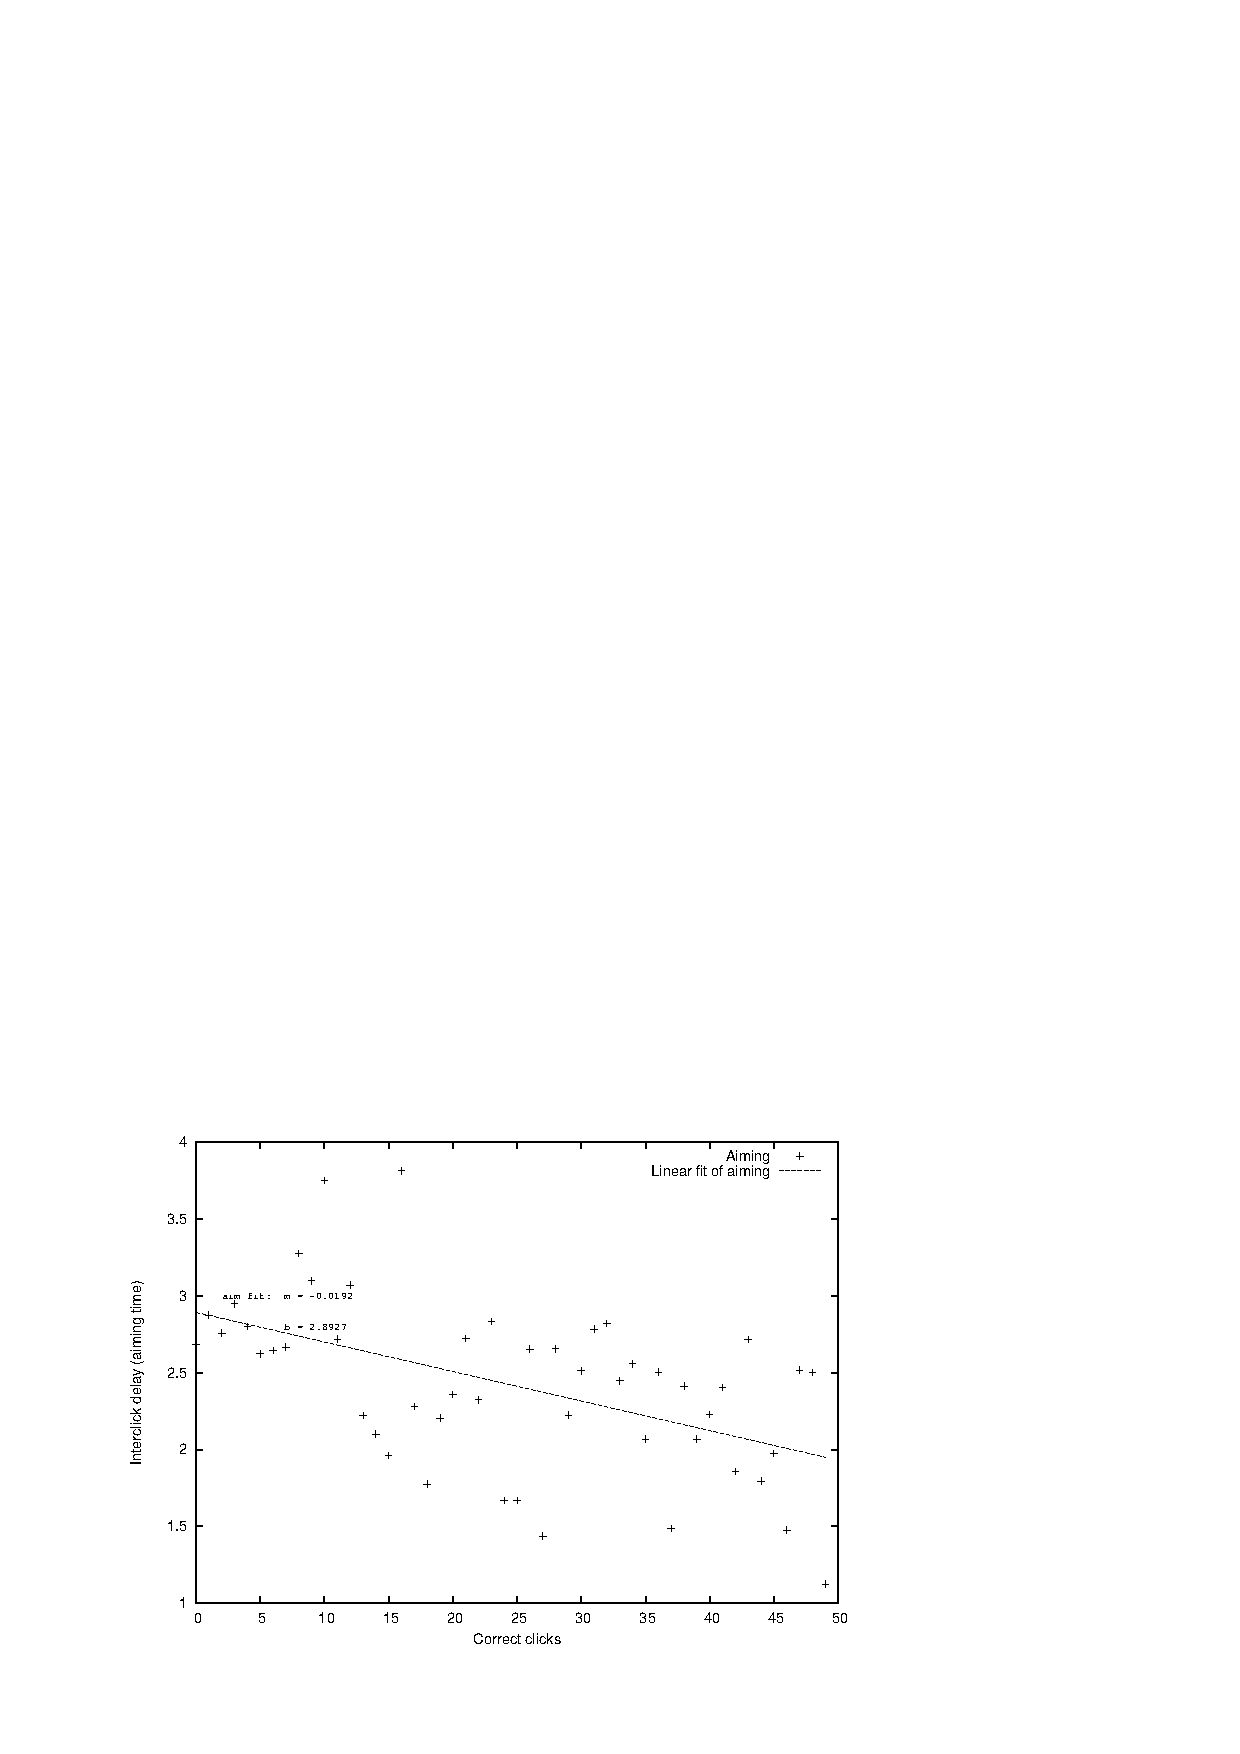
\includegraphics[width=0.6\textwidth]{img/aiming_time_progress.pdf}
\caption{Graf zlepšení práce v závisloti na čase.}
\label{fig:basicidea}
\end{figure}



\newpage

\appendix

\section{Návrh zadání}\label{zadani}

{\it Název:}~{\bf Pokus o vytvoření jednoduchého 3D polohovacího zařízení.}
\begin{itemize}
\item{2 myši (nebo jiné polohovací zařízení), každá ovládá pozici na jedné
      rovině ($xy$, $xz$ či $yz$).}
\item{Hlavní fór by byl v tom, že by i druhá myš (a ne jen kurzor v rovině kolmé
      k desce stolu) fyzicky jezdila po rovině kolmé k desce stolu.}
\item{Vhodnou kombinací vstupů z těchto 2 myší lze určit bod v 3D a případně
      s ním manipulovat (pozice na ose společné pro obě použité roviny
      by se určila jako průměr souřadnic).}
\item{Možné módy (možno měnit např. kombinací stisků tlačítek na myši):}
    \begin{itemize}
    \item{{\bf základní}\,--\,posunování 3D kurzoru v prostoru,
            tlačítkem se provede výběr nejbližšího objektu}
    \item{{\bf rotační}\,--\,rotace vybraného objektu pomocí např. pomocí
            \uv{circullar-scrolling}}
    \item{{\bf morfní}\,--\,změna nějakého atributu objektu
            (velikost, barva, tvar, ...)}
    \end{itemize}
\item{Nebo celé úplně jinak, cílem by bylo zkoumat schopnosti interakce
        takovéhoto HW zařízení.}
\item{K demonstraci by sloužila např. hra 3D piškvorky (pro jednoduchost
        by bylo implementováno pouze označování políček a ne logika
        hry\,--\,cílem projektu by nebylo vytvořit hru 3D piškvorky,
        ale \uv{prověření zařízení pro práci ve 3D}).}
\item{{\it openGL}}
\item{Možné využití (jen co mě napadlo): modelování 3D scény, hry,
        ovládání jeřábu, \ldots}
\end{itemize}

% \bibliographystyle{plain}
% \bibliography{itu}

\end{document}
